\chapter{Конструкторский раздел}
\label{cha:design}

\section{Конечный автомат SMTP-сессии на сервере}

Конечный автомат SMTP-сессии представлен на рисунке~\ref{fig:fsm}.

\begin{figure}
\centering
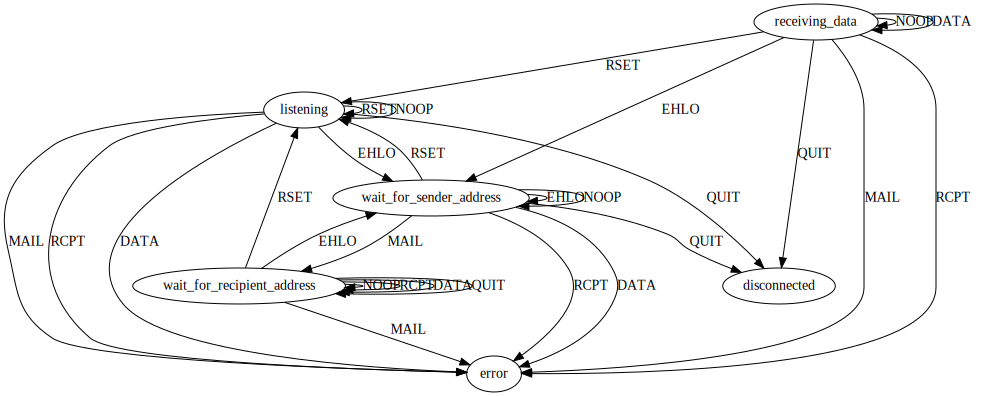
\includegraphics[width=\textwidth]{inc/fsm.pdf}
\caption{Конечный автомат SMTP-сессии}
\label{fig:fsm}
\end{figure}

Init -- начальное состояние.
После приветствия клиента выполняется переход по событию begin.
Далее сервер принимает команды клиента.
Любая ошибка вызывает событие error.
Done -- конечное состояние при корректном завершении сессии.
Invalid -- конечное состояние при таймауте (событие timeout).

События ehlo, rset, mail, rcpt, data, quit возникают при получении соответствующей команды от клиента.
More data -- при получении очередной строки данных.
Data end -- при получении маркера конца данных.
Переход в следующее выполняется при успешном завершении обработчика команды.

\section{Синтаксис поддерживаемых комманд протокола SMTP}

Сервер поддерживает следующие команды:
\begin{itemize}
\item Команды EHLO и HELO

\verb;^(?i:ehlo|helo)(?:\s*(<domain>))?\s*\r\n;

\verb;<domain> = [^/]+; -- домен клиента.

\item Команда RSET

\verb;^(?i:rset).*\r\n;

\item Команда MAIL

\verb;^(?i:mail from):\s*<(?:[^:]*:)?(<reverse-path>)>.*\r\n;

\verb;<reverse-path> = [^>]+; -- адрес отправителя.

\item Команда RCPT

\verb;^(?i:rcpt to):\s*<(?:[^:]*:)?(<forward-path>)>.*\r\n;

\verb;<forward-path> = [^>]+; -- адрес получателя.

\item Команда DATA

\verb;^(?i:data).*\r\n;

\item Строка данных

\verb;^.*\r\n;

\item Маркер конца данных

\verb;^\.\r\n;

\item Команда QUIT

\verb;^(?i:quit).*\r\n;

\item Команда VRFY

\verb;^(?i:vrfy).*\r\n;

\end{itemize}

\section{Сценарии взаимодействия с сервером}

Основной сценарий SMTP-сессии состоит в выполнении почтовой транзакции (см. рисунок~{fig:session}).
При этом взаимодействуют главный и подчиненный процессы, которые в свою очередь пишут в журнал.
Подчиненный процесс работает с хранилищем данных -- Maildir.

\begin{figure}[ht!]
	\centering
	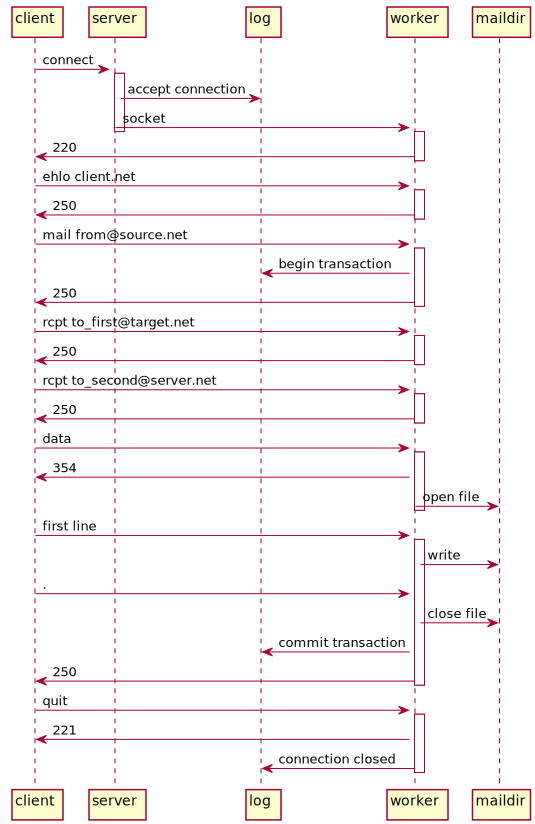
\includegraphics[width=\textwidth]{inc/session.pdf}
	\caption{Сценарий взаимодействия подсистем во время SMTP-сессии}
	\label{fig:session}
\end{figure}

\section{Структуры данных}

\subsection{Структура контекста SMTP-сессии}

\begin{verbatim}
typedef struct context {
    const settings_t *settings;
    log_t *log;
    te_smtp_server_state state;
    buffer_t in_message;
    buffer_tailq_t out_message_queue;
    int socket;
    int is_wait_transition;
    char command[COMMAND_SIZE];
    char uuid[UUID_STRING_SIZE];
    transaction_t transaction;
    struct timeval init_time;
    struct timeval last_action_time;
} context_t;
\end{verbatim}

Используется для хранения состояния SMTP сессии и всех используемых данных.
Поле \verb;settings; содержит общие настройки сервера,
\verb;log; -- данные модуля логирования,
\verb;state; -- состояние конечного автомата,
\verb;in_message; -- буфер с полученными от клиента сообщениями,
\verb;out_message_queue; -- очередь из буферов сообщений для отправки клиенту,
\verb;socket; -- дескриптор клиентского сокета,
\verb;is_wait_transition; -- флаг неполного завершения перехода в конечном автомате,
\verb;command; -- последняя полученная команда от клиента,
\verb;uuid; -- уникальный идентификатор сессии,
\verb;transaction; -- данные о почтовой транзакции,
\verb;init_time; -- время начала сессии (в подчиненном процессе),
\verb;last_action_time; -- время последней операции по обработке сессии.

\subsection{Структура почтовой транзакции}

\begin{verbatim}
typedef struct transaction {
    const settings_t *settings;
    log_t *log;
    char data_filename[PATH_SIZE];
    char *domain;
    char *header;
    char *reverse_path;
    int is_active;
    int sock;
    recipient_list_t recipient_list;
    struct aiocb aiocb;
    struct recipient *first_recipient;
} transaction_t;
\end{verbatim}

Используется для хранения состояния почтовой транзакции.
Поле \verb;data_filename; содержит имя файла для записи письма,
\verb;domain; -- домен клиента,
\verb;header; -- сгенерированный заголовок Received,
\verb;reverse_path; -- адрес отправителя,
\verb;is_active; -- флаг выполнения транзакции,
\verb;sock; -- дескриптор клиентского сокета,
\verb;recipient_list; -- список получаетелей,
\verb;aiocb; -- данные модуля для асинхронной записи на диск,
\verb;first_recipient; -- первый получатель.

\subsection{Структура получателя письма}

\begin{verbatim}
typedef struct recipient {
    char *address;
    maildir_t maildir;
} recipient_t;
\end{verbatim}

Используется для информации о получателе.
Поле \verb;address; содержит почтовый адрес,
\verb;maildir; -- данные о хранилище писем на сервере.

\subsection{Структура хранилища писем Maildir}

\begin{verbatim}
typedef struct maildir {
    char path[PATH_SIZE];
} maildir_t;
\end{verbatim}

Используется для хранения пути к директории.

\subsection{Структура буфера данных}

\begin{verbatim}
typedef struct buffer {
    char *data;
    size_t read_pos;
    size_t write_pos;
    size_t size;
} buffer_t;
\end{verbatim}

Используется для хранения сообщений клиента, прочитанных из сокета.
Поле \verb;data; содержит указатель на начало буфера,
\verb;read_pos; -- текущую позицию чтения,
\verb;write_pos; -- текущую позицию записи,
\verb;size; -- размер буфера.

\section{Алгоритм обработки соединений}

Алгоритм работы главного процесса:
\begin{verbatim}
listen_socket = soсket()
bind(listen_socket, address, port)
listen(listen_socket)
worker_pool = init_worker_pool(worker_pool_size)
while not is_need_exit():
    socket = accept()
    worker = select_worker(worker_pool)
    delegate_socket(worker, socket)
destroy_worker_pool(worker_pool)
close(listen_socket)
\end{verbatim}

Алгоритм работы подчиненного процесса:
\begin{verbatim}
while not is_need_exit():
    poll_sockets = empty list
    foreach socket, context in context_table:
        add socket to poll_sockets
    poll(poll_sockets)
    foreach socket in poll_sockets:
        if socket == pipe_socket:
            if socket flag HUP or ERR set:
                exit()
            if socket flag IN set:
                client_socket = read_client_socket(socket)
                context_table[client_socket] = create_context()
        else:
            if socket flag HUP or ERR set:
                remove context_table[socket]
                close(socket)
            else:
                if socket flag IN set:
                    recv(socket, context_table[socket].in_message)
                process_client(context)
                if socket flag OUT set:
                    out_message = top(context_table[socket].out_message_queue)
                    send(socket, out_message)
                    if out_message.read_pos == out_message.write_pos:
                        pop_front(context_table[socket].out_message_queue)
\end{verbatim}
